\documentclass[12pt,a4paper]{article}

\title{NFTsim User Manual}
\author{Complex Systems\\School of Physics\\University of Sydney}
\date{\today}


\usepackage{listings}
\usepackage{hyperref}
\usepackage{graphicx,xcolor}
\usepackage[top=2cm,bottom=3cm,left=2.2cm,right=2.2cm]{geometry}
\usepackage{multirow}
\usepackage{amsmath}
\usepackage{tikz}
\usepackage{placeins}
\usepackage{fancyhdr}
\usepackage{textcomp}
\usetikzlibrary{shapes,arrows,positioning}

\usepackage{tocloft}
\setlength\cftparskip{4pt}
\setlength{\cftbeforesecskip}{4pt}

\pagestyle{fancy}
\parindent=0.0cm
\parskip=0.5cm
\fancyhf{}
\lhead{{\em NFTsim} User Guide}
\rfoot{\thepage}
\lfoot{{\scriptsize \textcopyright\ Brain Dynamics Group, University of Sydney 2015}}

\footskip=1.0cm

\lstset{
basicstyle=\small\ttfamily,
frame=single,           % adds a frame around the code
breaklines=true,        % sets automatic line breaking
breakatwhitespace=tru,  % sets if automatic breaks should only happen at whitespace
aboveskip=12pt,
belowskip=0pt,
xleftmargin=1ex
}

\newcommand{\type}[1]{{\small\small\tt #1} }

\newcommand{\NF}[0]{\type{NFTsim}}

\graphicspath{{Figure/}}

\newcommand{\alert}[1]{ \colorbox{pink}{\parbox{\textwidth}{#1} } }

\renewcommand{\familydefault}{\sfdefault}


\definecolor{skyblue}{hsb:rgb}{0.95,0.97,1}
\newsavebox{\mybox}
\newenvironment{worked_example}
{\begin{lrbox}{\mybox}\begin{minipage}{\textwidth}}
{\end{minipage}\end{lrbox}\fcolorbox{black}{skyblue}{\parbox{\textwidth}{{\bf Worked example}\\\\\usebox{\mybox}}}}


\begin{document}

\section*{NFTsim User Guide}

\NF is a \type{C++} program developed by the Brain Dynamics Group at the University of Sydney, which solves the neural field model of Robinson et al. It is one of a core group of software analysis packages we have developed for our research.

The role of \NF is to integrate neural field equations to predict neural activity in neural field models with arbitrary numbers of populations and connections between them. As such, \NF can be viewed as a generalized neural field integrator that enables users to:

\begin{enumerate}
    \item Specify an arbitrary population model: an arbitrary number of populations and connections them may be specified;
    \item Choose different types of populations, including neural or stimulus populations. For each neural population, the type of firing response, dendritic response type may be specified.
    \item Choose different types of connections, including the type of axonal propagation, and synaptic coupling.
    \item For each object, specify the parameter values.
\end{enumerate}

This users guide covers the obtaining and setting up (Sec.~\ref{sec:obtain}), configuring (Sec.~\ref{sec:config}) and launching of \NF (Sec.~\ref{sec:running}), as well as postprocessing (Sec.~\ref{sec:analysis}) and tips and tricks (Sec.~\ref{sec:tips}).

Within this documentation, specific terminology as appeared in the computer is in \type{typewriter font}. Commands are denoted as
\begin{lstlisting}
Command to put in computer
\end{lstlisting}

% \begin{worked_example}
% If this is your first time setting up \NF, follow along with the worked examples in the shaded boxes. This will walk you through setting up and testing \NF.
% \end{worked_example}

\subsection*{Assumed knowledge}
To get the most out of \NF, you will require a working knowledge of neural field theory. In \NF, each neural field component is handled by an object:
\begin{align*}
    P &= \nu_{ab}\phi_{ab}, & \mathtt{Coupling}\\
    D_{ab}V_{ab} &= P, & \mathtt{Dendrite}\\
    Q_a &= S_a \big[\sum_b V_{ab} \big], & \mathtt{FiringResponse}\\
    \mathcal{D}_{ab}\phi_{ab} &= Q_b.&  \mathtt{Propagator}
\end{align*}
A detailed understanding of these equations is not essential to use \NF. However, you should be familiar with the roles of these components in neural field models. TODO - GO HERE TO FIND OUT MORE

\NF input and output files are both written in plain text, with syntax detailed in this manual. The analysis routines included with \NF are written in Matlab, and this documentation assumes that you are already familiar with basic use of Matlab. TODO - GO HERE TO FIND OUT MORE
%\pagebreak
%\tableofcontents

\section{Obtaining and setting up NFTsim}
\label{sec:obtain}

\subsection{Obtaining NFTsim}

\NF can be obtained from our website, \url{http://sydney.edu.au/science/physics/research/complex-systems/brain-dynamics/software.shtml}. As per the license agreement, users are not permitted to redistribute this program to other individuals or organizations - they should download NFTsim directly so as to have the most recent version, including any corrections.

\subsection{Directory layout}

All of the files associated with \NF are contained in a directory called \type{nftsim}. This directory is referred to as the `root directory', and it contains the following:

\begin{tabular}{l p{13cm}}
\type{src/}& \type{C++} source code.\\
\type{(obj/)}& This directory is created during compilation and stores intermediate object code.\\
\type{(dep/)}& This directory is created during compilation and stores dependency information.\\
\type{(bin/)}& The compiled binary \type{nftsim} is created here.\\
\type{configs/}& Stores example configuration files for \NF.\\
\type{doc/}& Contains this manual and the reference manual once it's built.\\
\type{+nf/}& Matlab package directory containing \NF helper scripts.\\
\type{test/}& Directory for development testing and is irrelevant for users.\\
\end{tabular}

\subsection{Compiling NFTsim}
\label{sec:compiling}
You can compile NFTsim simply by running

\begin{lstlisting}
make
\end{lstlisting}

from the root directory. The compiler command is specified in \type{Makefile}. On Linux this defaults to \type{g++} and on Mac it defaults to \type{clang++}. To run \NF on Windows, we suggest cross-compiling using MinGW on a Unix-like system. Example compiler flags for this are included in \type{Makefile}. Compiling with the Microsoft Visual \type{C++} compiler has not been tested.

The \type{Makefile} also provides a number of additional commands. This documentation along with the reference-manual can be generated by running
\begin{lstlisting}
make docs
\end{lstlisting}
which will recompile the \LaTeX\ files in the \type{doc/} directory if they've been updated since the last time this .pdf was generated, and run doxygen to generate the reference-manual from the source code. The reference manual can then be viewed by pointing your web-browser at

\begin{lstlisting}
doc/html/index.html
\end{lstlisting}

To delete the dependency files, object code, and temporary \LaTeX\ files (e.g., to perform a clean compile of the program), you can use
\begin{lstlisting}
make clean
\end{lstlisting}
which will delete the \type{dep/*.d} and \type{obj/*.o} files, as well as the temporary \LaTeX\ files in \type{doc/}. For a list of additional make targets, including brief descriptions of their function, run
\begin{lstlisting}
make help
\end{lstlisting}

\section{Running NFTsim}
\label{sec:running}
You can run \NF directly using

\begin{lstlisting}
./bin/nftsim
\end{lstlisting}

from the main \NF directory. For ease of use, you may consider adding the \type{nftsim} binary to your system path.

By default, \NF will check if a configuration file called \type{nftsim.conf} exists in the current directory. If this file exists, \NF will run it and write output to the file \type{nftsim.output} in the current directory. When these default files are used, a warning is displayed:

\begin{lstlisting}
romesha@romeshalt: nftsim > ./bin/nftsim
Warning: Using nftsim.conf for input by default
Warning: Using nftsim.output for output by default
\end{lstlisting}

Note that NFTsim will overwrite the output file if it exists, so it is not a good idea to use \type{nftsim.output} for your work.

You can optionally provide an input file using the \type{-i} switch. For example,

\begin{lstlisting}
./bin/nftsim -i configs/example.conf
\end{lstlisting}

will use the configuration file \type{example.conf} within the \type{configs} directory, and will write output to \type{example.output} also in the \type{configs} directory. The output file name is generated by replacing the input file's suffix (\type{.conf}) with \type{.output}.

Or you can also specify an output file, using the \type{-o} switch. For example, if you want your configuration files and output data to be in different directories,

\begin{lstlisting}
./bin/nftsim -i configs/example.conf -o example.output
\end{lstlisting}

will use the configuration file \type{example.conf} within the \type{configs} directory, and will write output to \type{example.output} in the current directory.

A list of available switches can be displayed by using the \type{-h} or \type{--help} option i.e., \type{./bin/nftsim -h}

\subsection{Writing a configuration file}
\label{sec:config}

\NF allows an arbitrary number of populations and connections between them, with all objects taking arbitrary parameter values. These are all configured via a configuration file. This section documents the specifications of configuration files, where we use \type{configs/example.conf} as an illustrative example.

To write a configuration file, follow these steps:
\begin{enumerate}
\item Determine your population model by drawing a schematic diagram, thereby constructing a connection matrix. An example is shown in Fig.~\ref{fig:cortical}.
\item Look up existing configuration files in \type{configs/}. By checking the comment located at the top of a configuration file, and also the connection matrix, a user should find the most suitable existing file to construct his own. This is less tedious (and less error prone) than writing a new one from scratch.
\item Specify the global parameters and connectivity matrix (Sec.~\ref{sec:global}).
\item Specify all populations (Sec.~\ref{sec:pop_conf}).
\item Specify all propagators (Sec.~\ref{sec:prop}).
\item Specify all couplings (Sec.~\ref{sec:coupling_conf}).
\item Specify all output requests (Sec.~\ref{sec:output_conf}).
\end{enumerate}

General rules on the entries within a configuration file:

\begin{enumerate}
    \item The structure of a configuration file is: 1) comment 2) global information 3) object specification 4) output specification.
    \item Object specification involves first specifying the object type. The syntax is the object identifier, followed by its type, then a hyphen:
        \begin{lstlisting}
Object 1: Type -
        \end{lstlisting}
        Then the object parameters are specified, following this pattern:
        \begin{lstlisting}
Object parameter: value
        \end{lstlisting}
    \item Most parameters are essential. Failure to provide these parameters would result in \NF terminating with an error message. A minority of the parameters are optional.
    \item The ordering of the parameters are important. Wrong parameter ordering results in \NF terminating with an error message.
    \item The configuration file is white-space independent, e.g., there can be either no spaces, many spaces, or new lines between parameters.
    \item For readability, users are encouraged to arrange parameter entries for different objects (via new lines and indentations) and aligning corresponding parameters between different objects.
    \item Tip for \type{vi} users: \type{./Helper\_scripts/nftsim.vim} implements syntax highlighting for configuration files in \type{vi}. See comments within for installation instructions.
\end{enumerate}

\subsubsection{Example configuration}
The remainder of this section refers to an example configuration for the illustrative example system shown in Fig.~\ref{fig:cortical}. The corresponding configuration file is also shown below. This configuration file is included in the repository as \type{configs/cortex.conf} and can be run from the \NF repository root using

\begin{lstlisting}
./bin/nftsim -i configs/cortex.conf -o cortex.output
\end{lstlisting}

{\em It is recommended that you open \type{configs/cortex.conf} to read in conjunction with this section of the manual.}
\vspace{24pt}

\begin{figure}[h!]
\begin{center}
\tikzstyle{block} = [draw,text width=3em,text centered,minimum height=2em]
\tikzstyle{line} = [draw, -latex']
\begin{tikzpicture}[node distance = 1cm and 2cm, auto]
    \node[block] (epsilon) {$\epsilon$};
    \node[block, below= of epsilon] (iota) {$\iota$};
    \node[block, right= of epsilon] (e) {e};
    \node[block, right= of iota] (i) {i};
    \draw [->] (epsilon)--(e) node[midway] {1};
    \draw [->] (e) to[loop right] node[midway] {2} (e);
    \draw [->] ([xshift=-0.3cm]i.north)--([xshift=-0.3cm]e.south) node[midway] {3};
    \draw [->] (iota)--(i) node[midway] {4};
    \draw [->] ([xshift=0.3cm]e.south)--([xshift=0.3cm]i.north) node[midway] {5};
    \draw [->] (i) to[loop right] node[midway] {6} (i);
\end{tikzpicture}
\end{center}
\vspace{0.2cm}
\begin{center}
\begin{tabular}{ l l l l l }
    From:& $\epsilon$ & $\iota$ & e & i \\
    To $\epsilon$:& 0 & 0 & 0 & 0 \\
    To $\iota$:& 0 & 0 & 0 & 0 \\
    To e:& 1 & 0 & 2 & 3 \\
    To i:& 0 & 4 & 5 & 6
\end{tabular}
\end{center}
\caption{Top: schematic diagram of a purely cortical population model comprising excitatory and inhibitory populations, as well as two stimulus populations; each arrow indicates a connection between populations, so that each stimulus connects to a cortical population, and each cortical population connects to all cortical populations. Bottom: connection matrix indicating the connections between populations; zero indicates no connection, and a connection is indicated by a nonzero number, ordered top to bottom, left to right.}
\label{fig:cortical}
\end{figure}

\clearpage


\subsubsection{Global information}
\label{sec:global}

\begin{itemize}
\item {\em Initial comments}
\begin{lstlisting}
Example config file of cortical model with excitatory and inhibitory neurons
\end{lstlisting}
Any text before the text \type{Time:}, is disregarded by \NF and serves as comment, which is strongly recommended for all configuration files.
\item  {\em Integration time and timestep}
\begin{lstlisting}
Time: 10 Deltat: 1e-4
\end{lstlisting}
\type{Time} is the simulation duration in seconds.

\type{Deltat} is the time increment for each time step.
\item  {\em Grid size}
\begin{lstlisting}
Nodes: 4 Longside: 2
\end{lstlisting}
\type{Nodes} is the number of grid points in the spatial dimension per population of neurons. The code has been explicitly designed to have equal number of neurons per population.

\type{Longside} is an optional parameter, specifying the longside of the rectangular grid. If it is not supplied, it is assumed to be a square.

Both spatial dimensions have periodic boundary conditions, so that populations have the topology of a torus.

{\bf Note that the physical size of each neural population is specified in the definition of the population - see Sec.~\ref{sec:pop_conf}. For each population, $\Delta x$ is automatically computed based on the number of grid points and the physical size of the population.} This ensures that the physical size of the system does not change when the number of grid points is changed. When a wave propagator is included, the value of $\Delta x$ is automatically selected from the presynaptic population.

\item {\em Specifying connectivity}
\begin{lstlisting}
Connection matrix:
From: 1 2 3 4
To 1: 0 0 0 0
To 2: 0 0 0 0
To 3: 1 0 2 3
To 4: 0 4 5 6
\end{lstlisting}
We next specify a square connection matrix, where each entry is the connection from the column population to the row population. Zero indicates no connection, while a nonzero number indicates a connection. This number must be indexed from top to bottom, left to right.

The size of this matrix determines the number of neural populations in the simulation. The number of nonzero connections determines the number of dendrites, couplings and propagators that will be present in the configuration file.
\end{itemize}

\subsubsection{Population data}
\label{sec:pop_conf}
This section contains population information sections. There are two types of neural populations: ordinary populations and stimulus populations:
\begin{description}

\item[Stimulus populations]\ \\

\NF identifies stimulus populations as populations which have no dendrites, i.e., the row for that population contains no nonzero elements.  Each stimulus population information section is as follows.
\begin{itemize}
    \item \begin{lstlisting}
Population 1: Stimulation
    \end{lstlisting}
    The identifier \type{Population 1} is required for cross-checking.

    The descriptor \type{Stimulation} is not parsed by \NF, but it is strongly recommended for human referencing.
    \item
    \begin{lstlisting}
Length: .5
    \end{lstlisting}
    The physical edge length of the population (which is a 2D sheet), in metres. This is used in \type{Wave} propagators and the \type{PSD} of \type{White} stimulus.
    \item
    \begin{lstlisting}
Stimulus: Const - Onset: 0
    \end{lstlisting}
    The identifier \type{Stimulus} is required for cross-checking.

    This is followed by the type of stimulus, to be further elaborated below.

    Optional parameter \type{Onset} specifies the time [s] from the start of the simulation for the stimulus to begin. If unspecified, stimulus starts at time 0.

    Optional parameter \type{Duration} can be used to specify the length of time [s] that the stimulus is active. If unspecified the stimulus continues for the entire simulation.

    If optional parameter \type{Node} is specified, only the specified node indices will receive stimulation.

    Possible stimulus patterns:

    \vspace{5mm}
    \textbf{Constant}
    \begin{lstlisting}
Const - Mean: 5
    \end{lstlisting}

    \vspace{5mm}
    \textbf{PulseRect}
    \begin{lstlisting}
PulseRect - Amplitude: 1 Width: 2e-2 Frequency: 1 Pulses: 1
    \end{lstlisting}

    \vspace{5mm}
    \textbf{PulseSigmoid}
    \begin{lstlisting}
PulseSigmoid - Amplitude: 1 Width: 2e-2 Frequency: 1 Pulses: 1
    \end{lstlisting}

    \vspace{5mm}
    \textbf{Sine}
    \begin{lstlisting}
Sine - Amplitude: 1.0 Frequency: 2.0
    \end{lstlisting}

    \vspace{5mm}
    \textbf{White}

    Gaussian noise, characterized by the mean and standard deviation:
    \begin{lstlisting}
White - Mean: 1 StdDev: 20 Ranseed: 10
    \end{lstlisting}

    Alternatively, the power spectral density (PSD) may be specified instead of the standard deviation (StdDev). The advantage is that the PSD is invariant to change in \type{Deltat}, population \type{Length} and spatial \type{Nodes}. Given the PSD, \NF correctly calculates the standard deviation:
    \begin{lstlisting}
White - Mean: 1 PSD: 20 Ranseed: 10
    \end{lstlisting}

    In general, it is preferable to specify the noise using \texttt{PSD} rather than \texttt{StdDev}. 

    The random number generator may be specified in \type{Ranseed}. If a seed is not specified, an automatically-incremented seed will be used instead, so that multiple stimulus populations will have independent sequences. In general it is not necessary to set the seed manually unless different random numbers are required for otherwise identical runs.

    \vspace{5mm}
    \textbf{Superimposing stimuli}

    To superimpose 2 or more stimuli, begin with the keyword \type{Superimpose}, followed by the number of stimuli. Then list all the stimulus patterns and their parameters, with each stimulus pattern preceded by the keyword \type{Stimulus}.
    \begin{lstlisting}
Stimulus: Superimpose: 2
 Stimulus: White - Mean: 1 PSD: 1
 Stimulus: PulseRect - Onset: 0.5 Width: 2e-2 Frequency 1 Pulses: 1
    \end{lstlisting}

    \vspace{5mm}
    \textbf{Example stimuli-only.conf}

    \begin{lstlisting}
Time: 12 Deltat: 9.765625e-04
Nodes: 144

    Connection matrix:
From:  1 
To 1:  0


Population 1: Stimulation
Length: 0.5
 Stimulus: Superimpose: 2
 Stimulus: PulseRect - Onset: 2 Node: 62 Amplitude: 1.0 Width: 1.0 Period: 3 Pulses: 3
 Stimulus: PulseSigmoid - Onset: 2 Node: 42 Amplitude: 1.0 Width: 1.0 Period: 3 Pulses: 3 Sigma: 0.03125

Output: Node: 33 42 62 77 Start: 0
Population: 1
Dendrite:  
Propagator:
Coupling: 
    \end{lstlisting}
\begin{figure}[h]
\begin{center}
 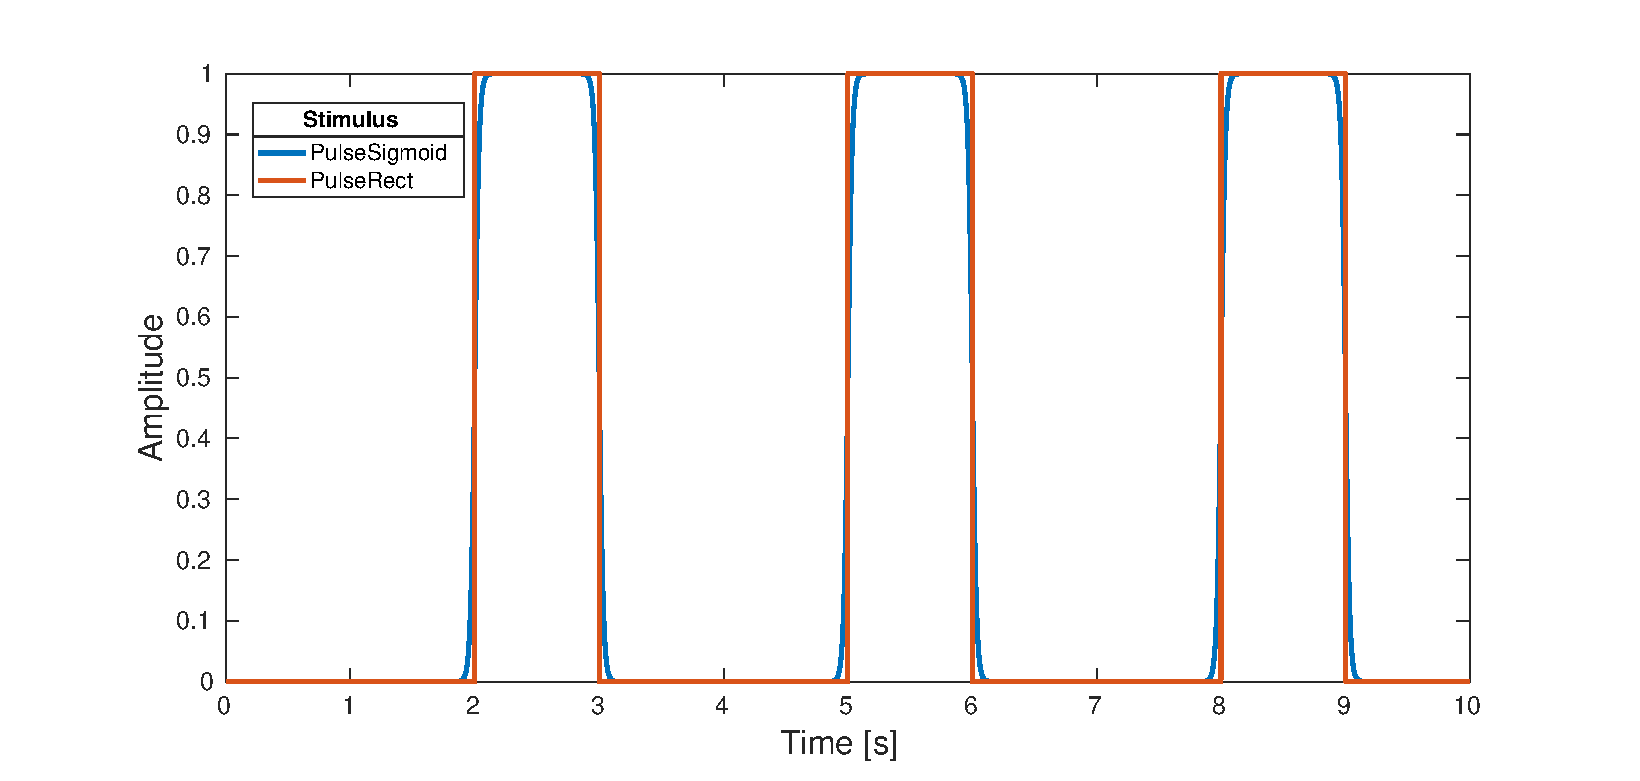
\includegraphics[width=\textwidth]{img/compare_pulsesigmoid_pulserect.eps}
 \caption{Note than in this example, the parameter \texttt{Onset} of \texttt{PulseSigmoid} is the time at which the sigmoid pulse reaches half of its range.}
\end{center}
\end{figure}

    \begin{lstlisting}
Time: 5 Deltat: 9.765625e-04
Nodes: 144

    Connection matrix:
From:  1 
To 1:  0


Population 1: Stimulation
Length: 0.5
 Stimulus: Superimpose: 4
 Stimulus: Sine - Onset: 1 Duration: 4 Node: 62 Amplitude: 1.0 Frequency: 0.5
 Stimulus: Sine - Onset: 2 Duration: 2 Node: 42 Amplitude: 1.0 Frequency: 2.0
 Stimulus: Sine - Onset: 1 Duration: 4 Node: 33 Amplitude: 1.0 Frequency: 0.5
 Stimulus: Sine - Onset: 2 Duration: 2 Node: 33 Amplitude: 1.0 Frequency: 2.0

Output: Node: 33 42 62 Start: 0
Population: 1
Dendrite:  
Propagator:
Coupling: 
    \end{lstlisting}
\begin{figure}[h]
\begin{center}
 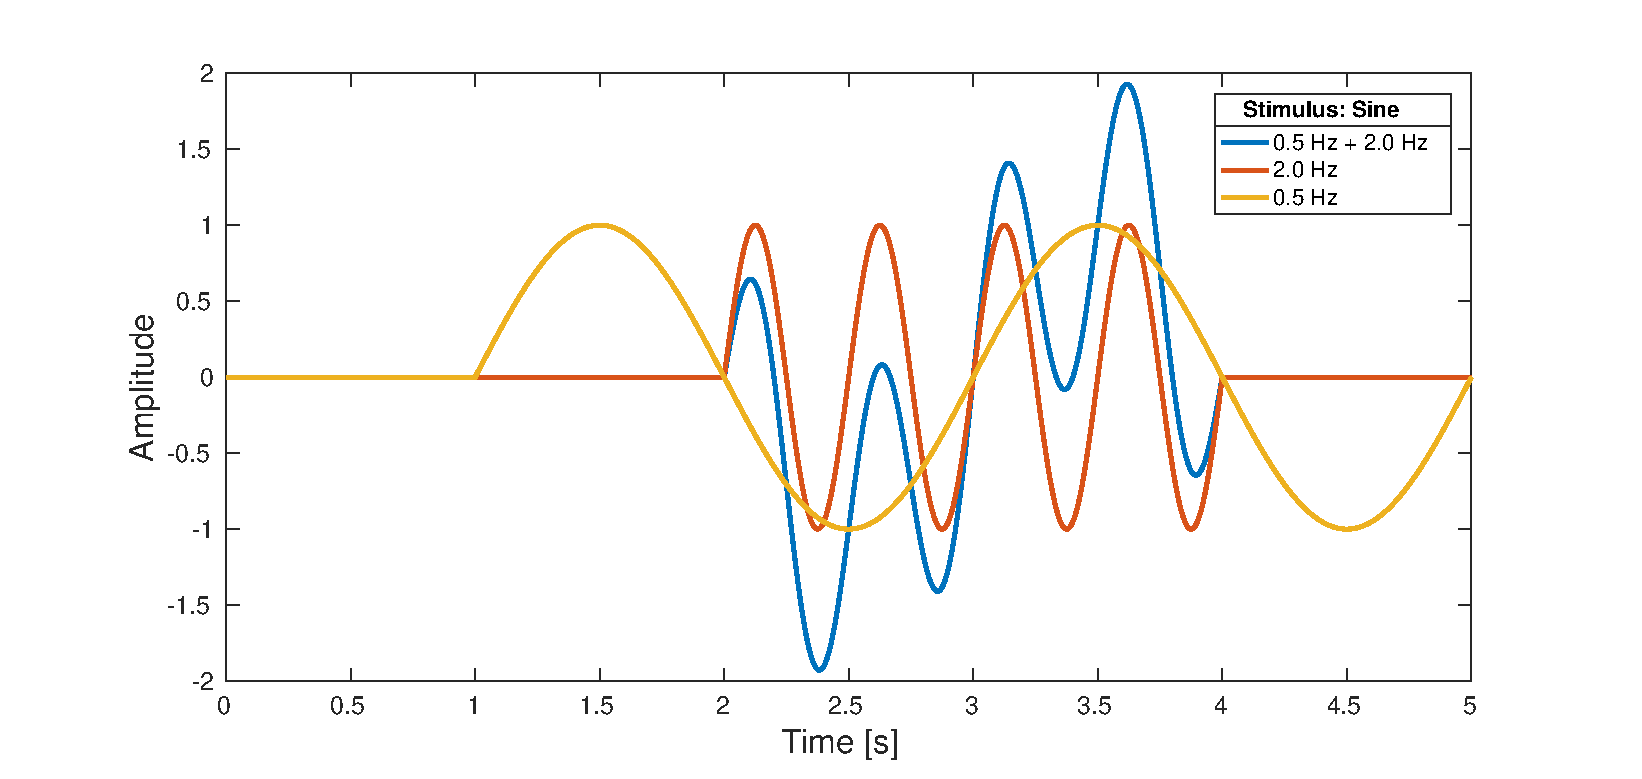
\includegraphics[width=\textwidth]{img/stimulus_sine.eps}
\end{center}
\end{figure}

    \end{itemize}
\item[Ordinary populations]\ \\
    Any non-stimulus population is an ordinary population.

    \begin{itemize}
    \item
    \begin{lstlisting}
Population 3: Excitory neurons
    \end{lstlisting}
    The identifier \type{Population 3} is required for cross-checking.

    The descriptor \type{Excitatory neurons} is not parsed by \NF, but it is strongly recommended for human referencing.
    \item
    \begin{lstlisting}
Q: 8.87145
    \end{lstlisting}
    The initial firing rate.
    \item
    \begin{lstlisting}
Firing: Sigmoid - Theta: 13e-3 Sigma: 3.8e-3 Qmax: 340
    \end{lstlisting}
    Specify the sigmoidal firing response of the population.

    \type{Sigma} is sometimes known as \(\tilde{\sigma}\). It is already scaled by \(\pi/\sqrt{3}\).

    Alternatively, you can specify a linear firing response by using
    \begin{lstlisting}
Firing: Linear - Gradient: 1 Intercept: 1
    \end{lstlisting}

    \item
    \begin{lstlisting}
Dendrite 1: V: Steady alpha: 83 beta: 769
    \end{lstlisting}
    The identifier \type{Dendrite 1}, where the number 1 is the presynaptic connection index, is required for cross-checking. Users should find that these indices are simply ordered as 1, 2, 3, 4, ...

    Optional parameter \type{V} may be used to specify the initial depolarization contribution from presynaptic activity. If unspecified, or set to \type{Steady}, \NF calculates the initial value by \(V_{ab}=\nu_{ab}\phi_{ab}\).

    \type{alpha} and \type{beta} are the parameters for the depolarization response.
    \end{itemize}
\end{description}

\subsubsection{Propagation data}
\label{sec:prop}
\begin{itemize}
\item
    \begin{lstlisting}
Propagator 1:
    \end{lstlisting}
    This identifier is required for cross-checking.
\item A propagator type is required at this point. Choices are \type{Map}, \type{Wave}, and \type{Harmonic}.
\begin{description}
    \item[Map]\ \\
    \begin{lstlisting}
Map - phi: Steady Tau: 0
    \end{lstlisting}
    This propagator is the mapping propagator where spatial spreading is negligible. Its form is given by
    \[\phi_{ab}({\bf r}, t) = Q_b ({\bf r}, t - \tau_{ab}).\]
    Optional parameter, \type{Tau}, is the axonal delay term. If unspecified, it is taken as zero. Since all propagators contain this object, its description is given below.

    Optional parameter \type{phi} may be used to specify the initial axonal firing rate. If unspecified, or set to \type{Steady}, \NF calculates the initial value by \(\phi_{ab}=Q_{b}\).

    \item[Wave]\ \\
    This propagator is the wave equation propagator governed by the equation
    \[\left[\frac{1}{\gamma_{ab}^2}\frac{d^2}{d t^2}+\frac{2}{\gamma_{ab}}\frac{d} {d t}+1 -r^2_{ab}\nabla^2 \right] \phi_{ab}({\bf r},t) =Q_b({\bf r},t-\tau_{ab}).\]

    \NF checks whether the Courant condition must be satisfied, i.e. \[\Delta t/\Delta x<\sqrt{2}/r_e\gamma_e,\] where $\Delta x$ is the population length per node.

    The propagator input is given by
    \begin{lstlisting}
Wave - phi: Steady Tau: 0 Range: 80e-3 gamma: 116
    \end{lstlisting}

    Optional parameter \type{phi} may be used to specify the initial axonal firing rate. If unspecified, or set to \type{Steady}, \NF calculates the initial value by \(\phi_{ab}=Q_{b}\).

    \type{Range} is $r_{ab}$ in the wave equation.

    \type{gamma} is the damping coefficient. Alternatively, \type{velocity} may be specified, and \type{gamma} is calculated via \(\gamma_{ab}=\mathrm{v}_{ab}/r_{ab}\).

    In case there is only one node, this degenerates into a \type{Harmonic} propagator.

    \item[Harmonic]
    This is a harmonic oscillator implementation of the damped wave equation, with no spatial variations:
    \[\left[\frac{1}{\gamma_{ab}^2}\frac{d^2}{d t^2}+\frac{2}{\gamma_{ab}}\frac{d} {d t}+1 \right] \phi_{ab}({\bf r},t) =Q_b({\bf r},t-\tau_{ab}).\]

    The input form is given by
    \begin{lstlisting}
Harmonic - phi: Steady Tau: 0 gamma: 116
    \end{lstlisting}

    \item[Tau]\ \\
    The axonal time delay between populations. If it is spatially homogeneous, then it is a number with units of seconds. If it is spatially inhomogeneous, then input \(n\) numbers, where \(n=\) \type{Nodes}.

\end{description}
\end{itemize}

\subsubsection{Coupling Classes}
\label{sec:coupling}



\begin{itemize}

\item The type of coupling between each pair of populations can be specified for separately. The coupling data is given as $n$ lines  corresponding to each nonzero connection in the connection matrix defined at the top of the file. Different types of coupling has their own input form.
\item \begin{lstlisting}
Coupling 1:
\end{lstlisting}
\item This syntax serves the purpose of an identifier for cross-checking. The following types of coupling are available:  \type{Map},  \type{Matrix},\type{Ramp}, \type{CaDP}, \type{BCM} and \type{DiffArctan}.
\begin{description}

\item[Map]\ \\
    Linear synaptic coupling with input parameter \type{nu}, constant time.
    This parameter may be a single number or take a vector of length
    \texttt{Nodes}, which allows for the expression of nonuniform models.
    \begin{lstlisting}
        Map - nu: 0.0012
    \end{lstlisting}
    where \type{nu} is the synaptic coupling parameter. In NFT, it corresponds
    to the product of the mean synaptic strength $s_{ab}$ and $N_{ab}$, the
    mean number of connections from cells of type $b$ to cells of type $a$.


\item[Ramp]\ \\
    Piecewise linear segments of increasing or decreasing \type{nu} can be
    specified by passing an array of nu values \type{nu} and array of time
    points \type{timepoints}, which together they specify the breakpoints  of
    a linear segment. Also, this coupling type assumes that at \type{t=0},
    \type{nu=nu[0]}, ie, the segment between \type{t=0} and timepoints[0] is
    constant. This behavior is appropriate to let the system reach a steady-state 
    or any other known stable attractor.

    \begin{lstlisting}
        Coupling 1:  Ramp - nu: 0.001525377176 0.001527 0.001527 0.00153 0.00153 0.001525377176 timepoints: 5 10 15 17.5 19.5 20
    \end{lstlisting}
    The resulting profile can be seen in Fig.~\ref{fig:coupling_ramp}.

    \begin{figure}[h]
        \begin{center}
            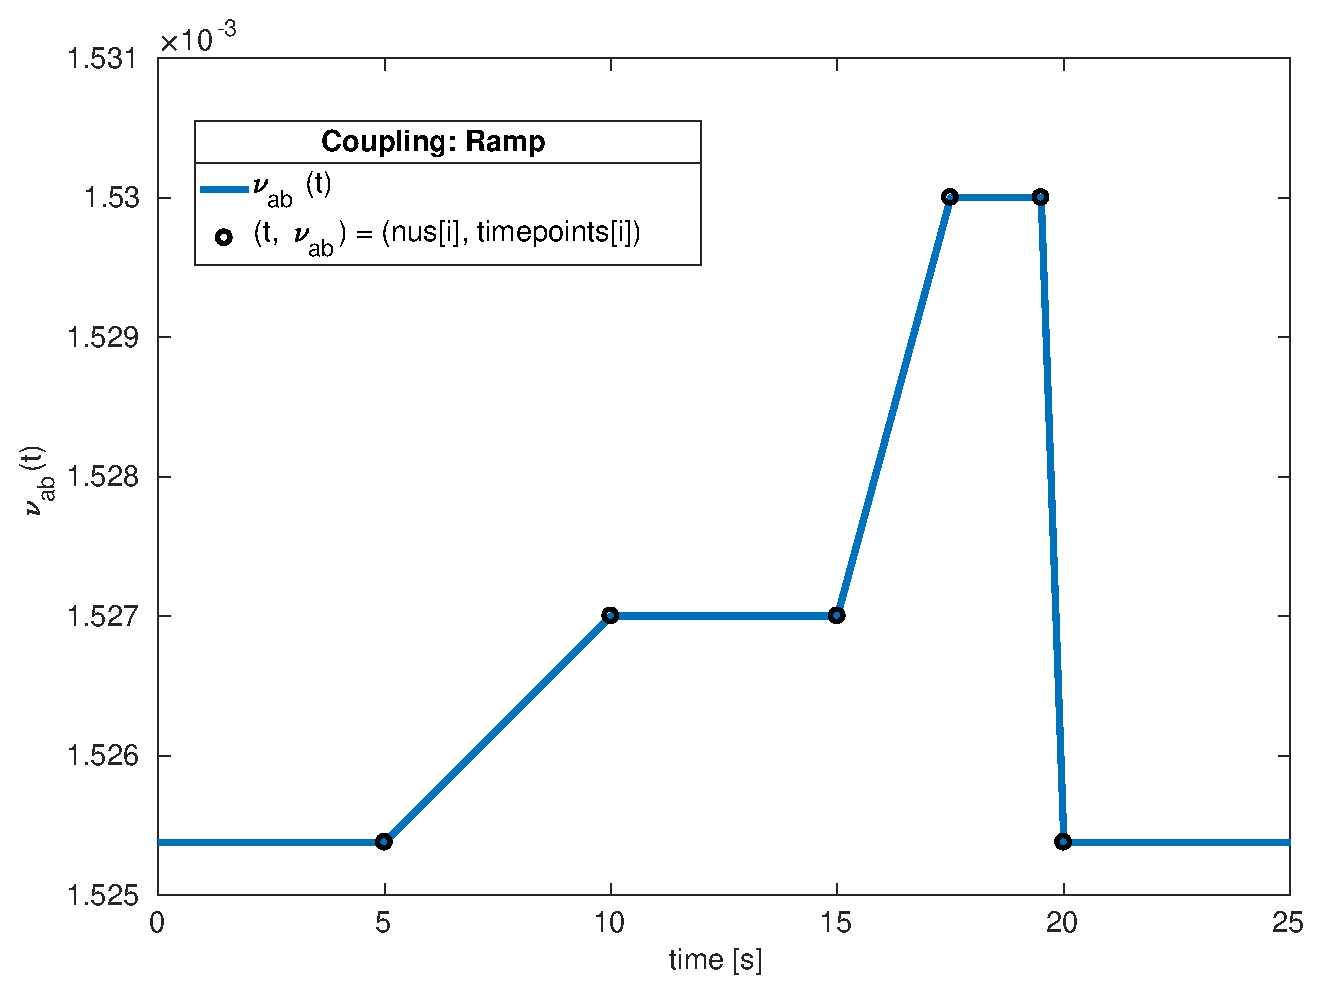
\includegraphics[width=\textwidth]{img/nftsim_coupling_ramp.eps}
            \caption{The resulting temporal profile of a $\nu_{ab}$ defined with \type{Ramp}. The circles highlight the breakpoints (\type{nu} and \type{timepoints}) specified in the configuration file.}
       \end{center}
       \label{fig:coupling_ramp}
    \end{figure}




    %\item[Modcouple]\ \\
    %The modulated synaptic coupling implements the Clearwater/Rennie modulation equation. The modulation is given by
    %\[ \nu (t) = \nu_0 \left[ ( 1 - \nu_{scal} ) e^{h(t)/k} + \nu_{scal} \right], \]
    %where $h(t)$ is the time low passed filtered form of the neuromodulators concentration $C(t)$ as given by
    %\[
    %\left\{ \frac{1}{\mu \lambda} \frac{d^2}{dt^2} +
    %\left[ \frac{1}{\nu}+ \frac{1}{\lambda}
    %\right]
    %\frac{d}{dt} + 1
    %\right\}
    %h(t) = C(t).
    %\]
    %The neuromodulator's concentration is in turn given by a user chosen stimulus form analogous to stimulus populations.

    %The remainder of the input form is specification of the output for $\nu$.  This takes an analogous form to the usual output data lines. The $\nu$ data is output to a file with filename \type{nftsim.synaptout.xx} where xx is an index number of the coupling.

    %An example Modcouple input form is given by
    %\begin{lstlisting}
%ModCoupling - Nuzero: 0.0002 Nuscal: 0.02 Mu: .1 Lambda: 1 k: .000001
%Concentration mode: 1  Time to start of Concentration: .01 Amplitude: .0001
%Pulse Duration: .2 Pulse repetition period: 40
%Number of traces: 100  Single/All: All nodes}
    %\end{lstlisting}

    \item[Matrix]\ \\

    The coupling may be expressed as a connection matrix, where the coupling
    strengths do not change with time. The format of the \texttt{nu} matrix is
    the same as the population connection matrix, each row is to the same
    node, each column is from the same node. When outputting, each specified
    outputting node output the indexed row.

    \begin{lstlisting}
nu:
  13e-6 0
  0 13e-6
    \end{lstlisting}

    \item[CaDP]\ \\
    Calcium dependent plasticity according to Fung and Robinson.
    \begin{lstlisting}
CaDP - nu: 13e-6 nu_max: 80e-6 Dth: .25e-6 Pth: .45e-6 xyth: 1e-4 x: 2.3e-2 y: 2e-2 B: 30e3 glu_0: 200e-6 gNMDA: 2e-3
    \end{lstlisting}

    \type{Dth} and \type{Pth} are the calcium-plasticity thresholds; \type{xyth}, \type{x} and \type{y} are the plasticity rates; \type{B}, \type{glu\_0} and \type{gNMDA} are NMDA receptor parameters.

    To use \type{CaDP}, glutamate dynamics must be specified for the postsynaptic population. In the end of the relevant population entry, append
    \begin{lstlisting}
Glutamate dynamics - Lambda: 150e-6 tGlu: 30e-3
    \end{lstlisting}
    \type{Lambda} is the glutamate concentration rise per presynaptic spike; \type{tGlu} is the decay timescale for glutamate dynamics.

    \item[BCM]\ \\
    Extends \type{CaDP} with metaplasticity according to Fung and Robinson. it has an additional parameter \type{t\_BCM}, the timescale of metaplasticity.
    \begin{lstlisting}
CaDP - nu: 13e-6 nu_max: 80e-6 Dth: .25e-6 Pth: .45e-6 xyth: 1e-4 x: 2.3e-2 y: 2e-2 B: 30e3 glu_0: 200e-6 gNMDA: 2e-3 t_BCM: 7
    \end{lstlisting}

    \item[DiffArctan]\ \\
    This type of coupling allows the connection strength $\nu_{ab}$ to vary as a function of time, such that $\nu$ can be smoothly ramped up and down.
    \begin{lstlisting}
DiffArctan - nu_min: 0.002  nu_max: 0.006  delta: 10  t_half_up:50  t_half_down:100
    \end{lstlisting}
where \type{nu\_min} and \type{nu\_max} are the min and max $\nu$'s respectively. \type{delta} determines the slope of the ramp (1/\type{delta}) and is the time interval in which the connection strength increases (decreases) from 0.25 to 0.75 of \type{nu\_max}. \type{t\_half\_up} and \type{t\_half\_down} are the half way times to maximum and minimum  amplitude, respectively.

\end{description}
\end{itemize}

\subsubsection{Output data}
\label{sec:output_conf}

\NF outputs field quantities (i.e. a neurodynamic quantity which takes a value for each node) with respect to nodes and time. By default, the output file is generated by replacing the input configuration file's suffix (\type{.conf}) with \type{.output}. The output file can be changed by launching the program with the \type{-o} switch.

\begin{itemize}
    \item \begin{lstlisting}
Output:
        \end{lstlisting}
Begin with the \type{Output} declaration.
\item \begin{lstlisting}
Node: 1 2
\end{lstlisting}
Enumerate all nodes to be outputted. If outputting all nodes, use shorthand \type{All}. If no nodes are specified, no nodes will be outputted.
\item \begin{lstlisting}
Start: 0 Interval: 1e-4
\end{lstlisting}
Optional parameters for the time to start output, and optional parameter for time interval between outputs.

If undefined, defaults, to 0 and \type{Deltat}, respectively.
\item \begin{lstlisting}
Population: 4.V
Dendrite: 5
Propagator: 1 4.phi
Coupling: 3.nu
\end{lstlisting}

\NF allows the user to specify which objects to output, by entering the appropriate object indices after the labels. For each object, it has some intrinsic fields that will be outputted; for example, \type{Coupling} outputs \type{nu}, whereas \type{CaDP} outputs \type{nu} and \type{Ca}.

For each entry, a field name may be appended after the index with a dot, so that only that field of the object is outputted. If no field name is specified for that entry, then all fields of that object is outputted.

If a specific field of an object is specified, but that field does not exist, \NF checks and returns an error.

\end{itemize}

\section{Analysis}
\label{sec:analysis}

\NF produces a single output file, unless a different name is manually specified this file's name is the same as the input file but with the suffix replaced by \type{.output}. The output file starts with a copy of the input file, to enable the output file to serve as a complete representation of the simulation. The simulation results follow a series of `\type{=}' characters. Example content in \type{nftsim.output} is
\begin{lstlisting}
=============================================
                Time            Propagator.2.phi
                                           0
1.00000000000000e-04    8.87145000000000e+00
\end{lstlisting}

Each column is a time series with its name indicated in the first line. The first column is always time, and in this example, the second column is \type{Propagator.2.phi}, indicating that it is $\phi_{ee}$ (when checked against connection matrix). The node number is indicated in the second line.

It is also worth noting that traces will be written in the order that they are specified. For example, if you write \type{Population: 3 1} then the columns in the output file will be arranged in this order.

\subsection{Matlab}
A number of Matlab functions are provided to make it easy to manipulate \NF data from within Matlab. The functions are generally self-documenting with comments at the start of the file. To use these functions, you should add the \NF root directory to your Matlab path. All of the programs in the \type{+nf} directory will then be available for use within Matlab as part of the \type{nf} package (e.g., typing \type{nf.run()} will execute the function specified in \type{+nf/run.m}).

\begin{figure}[b]
\begin{center}
\tikzstyle{pop_style} = [rectangle, draw, text width=6em, text centered, minimum height=4em]
\tikzstyle{couple_style} = [rectangle, draw, text width=6em, text centered, minimum height=4em,fill=gray!30]
\tikzstyle{line} = [draw, -latex']
\begin{tikzpicture}[node distance = 3cm, auto]
    \node[pop_style] (s1) {Decide model parameters};
    \node[couple_style,right of=s1] (s2) {Write configuration\\\type{nf.eirs()}};
    \node[pop_style,right of=s2] (s3) {Run \NF\\\type{nf.run()}};
    \node[pop_style,right of=s3] (s4) {Read configuration\\\type{nf.read()}};
    \node[pop_style,right of=s4] (s5) {Run analysis\\\type{nf.extract()}};

    \draw[line] (s1) -- (s2);
    \draw[line] (s2) -- (s3);
    \draw[line] (s3) -- (s4);
    \draw[line] (s4) -- (s5);

\end{tikzpicture}
\caption{Overview of typical \NF workflow, showing the roles of the various Matlab tools. For each step, the corresponding Matlab function is shown. Note that the configuration file contains different populations and couplings for different models of neural networks. The Matlab helper \type{nf.eirs()} is specific to the Robinson et. al. corticothalamic model, and is provided in the \type{cortiothalamic-model} software package (together with a number of other analysis routines specific to that model) available from the Brain Dynamics website.}
\label{fig:components}
\end{center}
\end{figure}

Essentially, an output file from \NF is read into a \type{nf} struct object in Matlab which simply contains all of the output from \NF in memory for easy access. Here is an example of a \type{nf} object:
\begin{lstlisting}
obj =
     fields: {'Propagator.1.phi'  'Propagator.3.phi'}
      nodes: {[1]  [1]}
       data: {[300000x1 double]  [300000x1 double]}
       time: [300000x1 double]
     deltat: 1.0000e-04
    npoints: 300000
\end{lstlisting}
\begin{itemize}
\item \type{fields} stores a record of which traces from \NF are present in the output file
\item \type{nodes} is a cell with the same size as \type{fields}, and records for each field present, the number of the node in the output.
\item \type{data} is a matrix storing the actual values of the traces.
\item \type{time} is a vector of time values, so that you can plot any of the data traces directly again \type{obj.time}.
\item \type{deltat} stores the temporal sampling rate.
\item \type{npoints} stores the total number of points in the output.
\end{itemize}

There are two ways to create the \type{nf} object. You can read the output file directly after executing \NF elsewhere

\begin{lstlisting}
obj = nf.read('nftsim.output')
\end{lstlisting}

or you can use the \type{nf.run} helper script to run the config file using \NF and automatically parse the output

\begin{lstlisting}
obj = nf.run('nftsim.conf')
\end{lstlisting}

%Using \type{nf\_run} means you will need to add \NF to your shell search path.

Several helper files are provided to manipulate the \type{nf} object. The two most important helpers are \type{nf.extract} and \type{nf.grid}. Often you want to extract a particular field from the \type{nf} object, for example, to examine the output from \type{Propagator.3.phi}. To do this directly with the nftsim struct, you would need to check the \type{fields} variable to find the index of the trace you wanted, and then extract it from the \type{data} field. In the previous example, \type{Propagator.3.phi} is the second trace. These expressions are identical:
\begin{lstlisting}
trace = obj.data{2};
trace = nf.extract(obj,'Propagator.3.phi')
\end{lstlisting}
\type{nf.extract} quickly becomes useful when there are many different fields. It is not case sensitive (so \type{propagator.3.phi} works as well). You can also specify using additional arguments to extract only a portion of the time series, and also to select a subset of nodes. Finally, you can also provide multiple traces to concatenate them into a single matrix. For example,
\begin{lstlisting}
trace = nf.extract(obj,'propagator.1.phi,propagator.3.phi');
\end{lstlisting}
will create a 300000$\times$2 matrix with both of the traces.

Finally, if you run \NF with multiple nodes, it typically solves the system of equations on a square grid. Therefore, if you have output for notes 1-400, this corresponds to a 20$\times$20 grid. \type{nf.grid} allows you to request a trace from the \type{nf} object and have it reshaped into a square grid. This lets you easily make surface plots of the data, or perform tasks that are spatially dependent.

One important task is computing the power spectrum as predicted by the linearized analytic equations. This can be achieved using \type{nf.spatial\_spectrum} which takes in an \type{nf} object and computes the power spectrum integrated over $k$ taking into account volume conduction.

\section{Development}

This section provides programming information about \NF for development extension and core logic. This section assumes a basic knowledge of \type{ANSI C++}, including object oriented programming, usage of template, and standard template library (STL). As our development takes place within a Git repository, a working knowledge of Git will significantly help.

A solid command of \underline{object-oriented programming} is an \underline{essential prerequisite}. Given the inevitable complexity arising from many developers and class relationships, good code structure and object-oriented programming principles must be adhered to whenever reasonable. One of the primary aims of object-oriented program as used by \NF is code reuse. Duplicated code, with subtle variations between them, is one of the best ways to introduce \underline{undetected numerical errors}. The ultimate consequence is erroneous publication and refactoring of the code. \underline{Code reuse} is one of the highest priorities. Sec.~\ref{sec:extension} contains methods for code reuse. When in doubt, read existing class implementations for examples, or contact the developers for assistance (\url{braindynamics@physics.usyd.edu.au}).

Here is a list of training resources:

\begin{itemize}
    \item Cpp resource
    \item Git resource
    \item OOP resource
\end{itemize}

\subsubsection{Development workflow}

We have adopted the {\em fork and pull} development model using GitHub. If you would like to contribute to \NF, set up your repository as follows:

\begin{enumerate}
    \item Make a private fork of the main repository.
    \item Clone your fork.
    \item Set an upstream remote pointing at the main \NF repository.
    \item Use \type{git pull upstream master} to merge changes from the main repository into the master branch of your working copy.
    \item We recommend using a branch in your fork for developing modifications
    \item When your feature is ready for integration into the main repository, submit a pull request on GitHub. Developers within the Brain Dynamics Group will then be able to review your code, check compatibility, and perform the merge.
\end{enumerate}

Note that you do not have write access to the main repository, so all changes must be proposed via pull requests. If your proposed changes are accepted, we may make modifications to ensure they integrate seamlessly with the rest of the program.

As discussed at the start of manual, \NF encapsulates each component of the model with an object: \type{Coupling}, \type{Dendrite}, \type{FiringResponse}, \type{Propagator}. The \type{Dendrite} and \type{FiringResponse} (and also \type{Timeseries}) are contained within \type{Population}.

Each object class may be overloaded for more sophisticated behaviour; for example, \type{Propagator} may be overloaded to perform wave propagation, or \type{Coupling} may be overloaded for synaptic plasticity.

\subsubsection{Coding style}

To maintain consistency within the \NF code base, we strongly encourage you to adhere to these programming conventions used throughout the project:

\begin{tabular}{ l l }
    Tabs:& two spaces.\\
    Braces:& the K\&R style.\\
    Class names:&UpperCamelCase\\
    Function names:&lowerCamelCase\\
    Variable names:&lowercase
\end{tabular}

When using the \type{C++} standard library, use the \type{using} directive to explicitly indicate the components you are using. For example,

\begin{lstlisting}
#include<vector>
using std::vector;
\end{lstlisting}

\subsection{Extending NFTsim via inheritance}
\label{sec:extension}

Most new functionalities may be introduced by inheriting existing classes and overloading appropriate functions, where the core classes are:

\begin{tabular}{l l l}
    Class&is Responsible for&Field\\
    \hline
    \type{Timeseries}&A function of time, predominantly used as stimulus.&\\
    \type{Dendrite}&Dendritic response.&$V_{ab}$\\
    \type{FiringResponse}&Firing response of population.&$V_a$\\
    \type{Population}&Contains \type{Timeseries}, \type{Dendrite}, and \type{FiringResponse}.&$Q_a$\\
    \type{Propagator}&Axonal firing propagation&$\phi_{ab}$\\
    \type{Tau}&Axonal propagation time latency&$\tau_{ab}$\\
    \type{Coupling}&Synaptic coupling&$\nu_{ab}$
\end{tabular}

Examples where these classes are inherited to provided new functionalities include:

\begin{tabular}{l l l}
    Derived class&Base class&Extension\\
    \hline
    \type{Wave}&\type{Propagator}&Wave propagation.\\
    \type{CaDP}&\type{Coupling}&Plastic synapse.\\
    \type{LongCoupling}&\type{Coupling}&Nonlocal synapse.
\end{tabular}

\subsubsection{Class hierarchy}
The diagram in Figure \ref{fig:classes} shows the inheritance hierarchy for the base NFTsim objects. Note that the \type{Array} class is a container object, and it is not necessary to interact with it directly. See Sec.~\ref{sec:array} for details.

\begin{figure}[h]
\label{fig:classes}
\tikzstyle{block} = [draw,text width=3em,text centered,minimum height=2em]
\tikzstyle{line} = [draw, -latex']

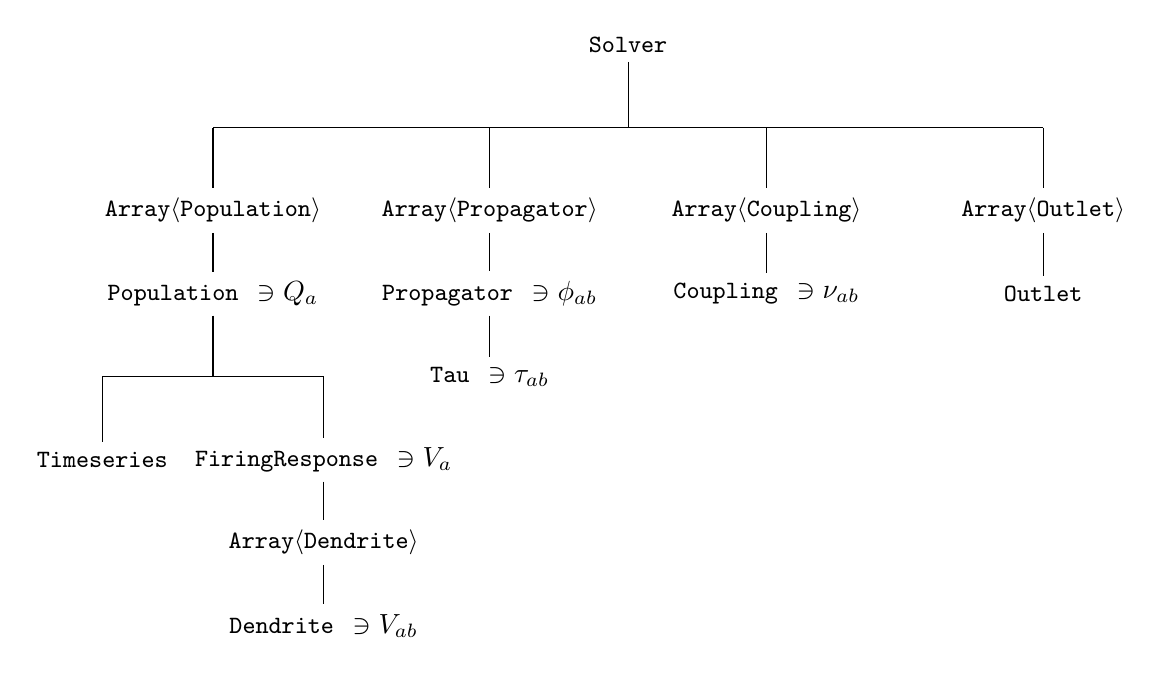
\begin{tikzpicture}[node distance = 3em, auto]
    \node[] (solver) {\type{Solver}};
    \coordinate[below of=solver,node distance=3em] (vsolver) {};
    \draw (solver) |- (vsolver);

    \coordinate[left of=vsolver,node distance=5em] (vpropag) {};
    \draw (vsolver) -- (vpropag);
    \coordinate[left of=vpropag,node distance=10em] (vpop) {};
    \draw (vpropag) -- (vpop);
    \coordinate[right of=vsolver,node distance=5em] (vcouple) {};
    \draw (vsolver) -- (vcouple);
    \coordinate[right of=vcouple,node distance=10em] (voutput) {};
    \draw (vcouple) -- (voutput);

    \node[below of=vpropag] (apropag) {\type{Array$\langle$Propagator$\rangle$}};
    \draw (vpropag) -| (apropag);
    \node[below of=vpop]    (apop) {\type{Array$\langle$Population$\rangle$}};
    \draw (vpop) -| (apop);
    \node[below of=vcouple] (acouple) {\type{Array$\langle$Coupling$\rangle$}};
    \draw (vcouple) -| (acouple);
    \node[below of=voutput] (aoutput) {\type{Array$\langle$Outlet$\rangle$}};
    \draw (voutput) -- (aoutput);

    \node[below of=apropag] (propagator) {\type{Propagator} $\ni \phi_{ab}$};
    \draw (apropag) -- (propagator);
    \node[below of=apop]    (pop) {\type{Population} $\ni Q_a$};
    \draw (apop) -- (pop);
    \node[below of=acouple] (coupling) {\type{Coupling} $\ni \nu_{ab}$};
    \draw (acouple) -- (coupling);
    \node[below of=aoutput] (output) {\type{Outlet}};
    \draw (aoutput) -- (output);

    \coordinate[below of=pop,node distance=3em](vpop){};
    \draw (pop) |- (vpop);
    \coordinate[left of=vpop,node distance=4em](vs){};
    \draw (vpop) |- (vs);
    \coordinate[right of=vpop,node distance=4em](vq){};
    \draw (vpop) |- (vq);

    \node[below of=vs,node distance=3em](s){\type{Timeseries}};
    \draw (vs) -- (s);
    \node[below of=vq,node distance=3em](q){\type{FiringResponse} $\ni V_a$};
    \draw (vq) -- (q);

    \node[below of=q](adendrite){\type{Array$\langle$Dendrite$\rangle$}};
    \draw (q) -- (adendrite);
    \node[below of=adendrite](dendrite){\type{Dendrite} $\ni V_{ab}$};
    \draw (adendrite) -- (dendrite);

    \node[below of=propagator,node distance=3em](tau){\type{Tau} $\ni \tau_{ab}$};
    \draw(propagator)--(tau);
\end{tikzpicture}
\tikzstyle{block} = [draw,text width=3em,text centered,minimum height=2em]
\tikzstyle{line} = [draw, -latex']
\caption{Schematic of the main class structures in \NF. Each line indicates that the bottom class is a member of the top class. The \type{a} $\ni b$ symbol indicates that the dynamical field $b(\mathbf{r},t)$ is a member of the class \type{a}. Inheritance structures are NOT illustrated.}
\end{figure}

\subsubsection{Procedure for implementing a new class}

Implementing a new class may be done using the following procedure:
\begin{enumerate}
    \item Identifying the core class to inherit (see above tables). Then look up the documentation of the appropriate base class from Sec.~\ref{sec:pop}--\ref{sec:dendrite}.
    \item Decide on the name of the class. Generally, it may be advantageous for the new name to refer to the base name, plus a terse description. For example, \type{LongCoupling} refers to its base class \type{Coupling}, with the additional description indicating that the new class has long range coupling. The file names should be the same as the class name, but all in lower case, for consistency.
    \item Overload appropriately the \type{init()} (see Sec.~\ref{sec:init}), \type{output()} (see Sec.~\ref{sec:output}), and \type{step()} functions. {\bf Do not} copy and paste code. Rather, use
        \begin{lstlisting}
BaseClass::function();
        \end{lstlisting}
    which will utilize the existing function in the base class. This will ensure that your derived class is updated if the base class changes.
    \item It is likely that differential equations are solved in the new class. \NF provides two classes, \type{DE} and \type{Stencil}, that solves spatially homogeneous differential equations, and spatially inhomogeneous equations, respectively. See Sec.~\ref{sec:diffeqn}.
    \item Register the new class as documented in Sec.~\ref{sec:pop}--\ref{sec:dendrite}.
    \item Write a configuration file that uses the new class. Or if the object may exhibit different types of behaviour under different parameter values, having one configuration file for each type of behaviour may be advantageous. Make sure that the configuration file has an appropriate comment.
\end{enumerate}

\subsection{NFTsim classes}

This section contains an overview of all of the base classes in NFTsim.

\subsubsection{Class NF}
\label{sec:nf}

All core classes are derived from the \type{NF} object. This abstract base class contains 3 member variables, and 3 interface methods:

\begin{tabular}{l l}
    \hline
Variable\\[6pt]
\hline
\type{nodes}&The number of nodes as specified from the configuration file.\\
\type{deltat}&The time increment per timestep in units of seconds.\\
\type{index}&The index associated with the object.\\[6pt]
\hline
Methods\\[6pt]
\hline
\type{init(Configf\& configf)}&Initializes the object with the config file.\\
 %\type{dump(Dumpf\& dumpf) const}&When the program terminates, all objects dump information into a dump file (\type{dumpf}) for later restart. \type{Dumpf} is an \type{ofstream}.\\
%\type{restart(Restartf\& restartf)}&Restarts the object in restart mode, \emph{in addition} to \type{init()}. The developer should have dumped all relevant information in dump, then reads it here.\\
\type{step(void)}&At each timestep, this function is called.\\
\type{output(Output\& output) const}&Specifies which fields to output.\\
\end{tabular}

All \type{NF} classes automatically handles the \type{ofstream::<<} and \type{ifstream::>>} operators.

When appropriate, the default constructor, copy constructor, and \type{operator=} should be made inaccessible by declaring them to be private.

\subsubsection{Population}
\label{sec:pop}

Models a neural population, which may be either a stimulus or normal population. If it has any \type{Dendrites}, i.e. it has presynaptic connections, then it is a normal population, and it is a stimulus if it does not have \type{Dendrites}.

In the former case, it contains the \type{FiringResponse} class and have a soma potential; in the latter case it contains the \type{Timeseries} class, and does not have a soma potential.

In either cases, the \type{Population} class has a keyring storing the firing rate history, coded as a 2D array plus an integer key.

Functions \type{sheetlength()} and \type{glu()} provides access to the physical length and glutamate concentration in synaptic cleft, respectively.

A population is ``settled" after \type{Population::init()} is called, after which no dendrites can be added, and the firing rate history cannot grow.

\subsubsection{Propagator}
\label{sec:propagator}

The \type{Propagator} class implements the axonal propagation as an identity map, i.e.
\[ \mathcal{D}_{ab} = 1. \]

To introduce more sophisticated axonal propagation, this class is inherited and overloaded.

The \type{Propagator} class provides a constant references to both presynaptic and postsynaptic populations.

Object \type{Tau} provides the axonal delay latency of propagator.

For spatially inhomogeneous propagators, class \type{Stencil} provides a Moore grid, as documented in Sec.~\ref{sec:stencil}.

To ``register" your propagator, look for the
\begin{lstlisting}
// PUT YOUR PROPAGATORS HERE
\end{lstlisting}
subsection in \type{solver.cpp}.

\subsubsection{Coupling}
\label{sec:coupling_conf}

The \type{Coupling} class manages \(\nu_{ab}\), which is constant in space and time.

To introduce synaptic plasticity, derive from this class.

The \type{Coupling} class provides a constant references to both presynaptic and postsynaptic populations. Glutamate concentration is also provided.

Function \type{excite()} indicates whether this is an excitatory coupling. Protected variable \type{pos} is $+1$ or $-1$, depending on the sign of \(\nu_{ab}\).

To ``register" your coupling, look for the
\begin{lstlisting}
// PUT YOUR COUPLINGS HERE
\end{lstlisting}
subsection in \type{solver.cpp}.

\subsubsection{FiringResponse}

To implement new firing response dynamics, inherit from class \type{FiringResponse}, where \type{init()} and \type{fire()} should be overloaded.

Object \type{dendrites} is an array of presynaptic \type{Dendrite}.

Objects \type{glu\_m} and \type{glu\_rk4} calculates glutamate concentration in the synaptic cleft, which is accessed via \type{glu()}.

To ``register" your firing response, look for the
\begin{lstlisting}
// PUT YOUR FIRING_RESPONSE HERE
\end{lstlisting}
subsection in \type{population.cpp}.

\subsubsection{Stimulus}

To implement new stimulus pattern, inherit from class \type{Timeseries}, where \type{init()} and \type{fire()} should be overloaded.

The time is provided via the variable \type{t}.

To ``register" your stimulus, look for the
\begin{lstlisting}
// PUT YOUR TIMEFUNCTION HERE
\end{lstlisting}
subsection in \type{timeseries.cpp}.

\subsubsection{Dendrite}
\label{sec:dendrite}

To implement new dendritic responses, inherit from class \type{Dendrite}.

References are provided for the presynaptic coupling and propagator.

To ``register" your dendritic response, look for the
\begin{lstlisting}
// PUT YOUR DENDRITE HERE
\end{lstlisting}
subsection in \type{firing\_response.cpp}.

\subsection{Adding variables to the configuration file}
\label{sec:init}

Your new class might require additional parameters in the configuration file. Input via the configuration file is implemented in the \type{init()} function, via \type{Configf}, which provides the following functions:
    \begin{enumerate}
        %\item \type{next()}: go to the next keyword.
        \item \type{param()}: go to the next keyword and reads in a variable. If the keyword is not found, barks and exits.
        \item \type{optional()}: same as param, but does not bark nor exit. The use of this function is discouraged, since it may introduce subtle bugs or human errors.
        \item \type{numbers()}: reads an arbitrary number of white-space separated numbers, returned in a \type{vector}.
        %\item \type{find()}: search a keyword and return the next variable as string.
    \end{enumerate}

    Sometimes the config file may search for either one parameter, OR another one. For example, \type{Wave} propagator accepts parameter \type{gamma} or \type{velocity} such that \type{gamma} = \type{velocity}/\type{range}, so that we may have either of these:
\begin{lstlisting}
Wave - Range: 80e-3 gamma: 116
\end{lstlisting}

\begin{lstlisting}
Wave - Range: 80e-3 velocity: 9.28
\end{lstlisting}

Then, we may use this pattern with \type{optional()} to achieve the desired effect:
\begin{lstlisting}
configf.param("Range",range);
if( !configf.optional("gamma",gamma) ) {
  double temp; configf.param("velocity",temp);
  gamma = temp/range;
}
\end{lstlisting}

\subsection{Adding variables to the output file}
\label{sec:output}

\NF outputs field variables at every timestep, where the user chooses which object to output via the configuration file, and the object chooses which fields to output in the \type{output()} function.

To output field solutions, overload \type{NF::output()} to write
\begin{lstlisting}
output.prefix("Object Name",index+1);
output("field1",field1);
output("field2",field2);
subobject1.output(output);
subobject2.output(output);
BaseClass::output(output);
\end{lstlisting}
or for a single output field,
\begin{lstlisting}
output("Object Name",index+1,"field1",field1);
\end{lstlisting}

where \type{field1}, and \type{field2} are \type{vector<double>} with size equal to the number of spatial nodes.

To output a single number, as opposed to a spatial field, use the function
\begin{lstlisting}
output.singleNode("Object Name",index+1,"field1",field1);
\end{lstlisting}
or
\begin{lstlisting}
output.singleNode("field1",field1);
\end{lstlisting}
where \type{field1} is a \type{vector<double>} of size 1.

\subsection{Tools for solving differential equations}
\label{sec:diffeqn}

Classes \type{DE} and \type{Integrator} (currently RK4 is implemented) are used to solve generic systems of ODEs, where the dynamical variables are homogeneous fields. For inhomogeneous DEs and spatial dependency, a 9-point stencil is provided in \type{Stencil}.

\subsubsection{Class DE}
\label{sec:de}

Class \type{DE} and \type{RK4} together solves ODEs of homogeneous fields.

To define your differential equation, declare a new class that inherits \type{DE}. Overload the \type{rhs()} function to define the differential equation. For example, the differential equation
\[
    F = m\frac{d^2x}{dt^2},
\]
is redefined as
\[
F = y_0,~x = y_1,~\frac{dx}{dt} = y_2,
\]
so that it can be formulated as a system of 1\textsuperscript{st} order differential equations
\[
    \frac{dy_0}{dt} = 0,~
    \frac{dy_1}{dt} = y_2,~
    \frac{dy_2}{dt} = my_0,
\]
with
\[
    y_0 = F,
\]
being an algebraic equation.

This can be defined in \type{NewDE::rhs()} as
\begin{lstlisting}
void NewDE::rhs( const vector<double>& y, vector<double>& dydt )
{
  // y = { F, x, dxdt }
  dydt[0] = 0;     // F, leave unchanged
  dydt[1] = y[2];  // x
  dydt[2] = m*y_0; // dxdt
}
\end{lstlisting}
where the comments are strongly recommended for readability.

Declare the number of differential equations (in this example, 3) in the constructor
\begin{lstlisting}
NewDE( int nodes, double deltat ) : DE(nodes,deltat,3) {}
\end{lstlisting}

To integrate \type{NewDE}, declare a pair of \type{DE} and \type{RK4} objects:
\begin{lstlisting}
NewDE de(nodes,deltat);
RK4 rk4(de);
\end{lstlisting}
then the differential equation may be solved via (usually done in \type{Class::step()})
\begin{lstlisting}
for( int i=0; i<nodes; i++ )
  de[0][i] = F; // algebraic equation
rk4.step();     // integrate differential equation by one step
\end{lstlisting}

Often, the \type{NewDE} class is incorporated in a \type{NewClass}. In such cases, it is advantageous to declare \type{NewDE} as \type{struct}, which is a class where all members are public by default, and have this new \type{NewDE} declared within \type{NewClass}, so that it is accessible within it. All parameters of the differential equation (in the example above, $m$) will then belong to \type{NewDE}.

Since \type{NewClass} has access to all members of \type{NewDE}, all initialization of \type{NewDE} may be done in \type{NewClass::NewClass()} and \type{NewClass::init()}.

Remember to redirect the interface and output variables to members of \type{NewDE}. For example,

\begin{lstlisting}
vector<double>& NewClass::x(void) const
{
  // original code from base class:
  // return _x;
  // new code in derived class replaces original x variable:
  return (*de)[1];
}
\end{lstlisting}

\begin{lstlisting}
void NewClass::output( Output& output ) const
{
  output.prefix("NewClass",index+1);
  // original code from base class:
  // output("x",_x);
  // new code in derived class replaces original x variable:
  output( "x",(*de)[1] );
}
\end{lstlisting}

To extend an existing \type{DE} class, for example extend \type{NewDE} to \type{New2DE}, inherit \type{New2DE} from \type{NewDE}. The \type{extend()} function allows the introduction of new differential equations and field variables.

\subsubsection{Stencil}
\label{sec:stencil}

Class \type{Stencil} provides Moore grid for spatially inhomogeneous calculations.

Given a stencil,
\begin{lstlisting}
Stencil stencil(nodes,longside,"Torus");
\end{lstlisting}

Use \type{operator=} to set the spatial field values of a \type{vector<double>}.

The stencil pointer can be set and get via the \type{set()} and \type{get()} functions, and incremented via \type{operator++}. The Moore grid can be read with
\begin{lstlisting}
stencil(nw); stencil(n); stencil(ne);
stencil( w); stencil(c); stencil( e);
stencil(sw); stencil(s); stencil(se);
\end{lstlisting}

\subsection{Core logic}

{\em Normal extension of \NF does not involve any modification of the core logic. Proposed to the core logic are unlikely to be accepted. This section is intended to provide context to understand the design of the base objects.}

One integration step of the model implements the following stages:

\begin{enumerate}
    \item  Dendritic response
    \item  Afferent summation.
    \item  Firing response/stimulus response.
    \item  Wave equation integration step which includes Q delay processing
    \item  Coupling response.
\end{enumerate}

Most of the computational {\em load} comes from integrating wave equations and harmonic oscillators within the dendritic responses. Most of the execution {\em time} is probably spent writing the output file.

Wave equations are integrated by explicit finite differences integration. A nine point spatial stencil is used to reduce high frequency spatial instabilities when driven by random noise. Other parts of code are unaffected by spatial geometry so this can be switched to irregular gridding easily.

Harmonic oscillators with dendritic response are integrated using a heavily strength reduced explicit direct integration assuming constant drive. This was more efficient than a constant drive RK4 algorithm which would not be fourth order in any case due to the constant drive. Rennie used a constant drive RK4 for his 1997 code.

\subsubsection{Class Array}
\label{sec:array}

\type{Array} is a container array to store objects that supports the \type{ofstream::<<} and \type{ifstream::>>} operators, as well as a \type{step(void)} function. This object typically is, but is not required to be, an \type{NF} object.

The \type{step(void)} function is equivalent to a \type{foreach(element).step()} in pseudocode. This function is encouraged over the use of \type{empty()}, \type{size()}, and \type{operator[]()}, which are discouraged to be used.

\subsubsection{Program flow}

Essentially, the program flow can be read from Fig.~\ref{fig:classes}, so that objects take priority from top to bottom, left to right, both in terms of initialization and stepping through each timestep. A more detailed description is given below, and the reader is referred to the source code for complete description.

We use the semicolon to denote a succession of functions/procedures, and \type{a()} $\Rightarrow$ \type{b()} symbol to denote function \type{b()} as content of function \type{a()}.

\begin{center}
\begin{tabular}{ | l l p{11cm} | }
\hline \\

\type{main()}& $\Rightarrow$ &Initialize the config file, dump file and output file;\\[6pt]
&&\type{Solver::init()};\type{Solver::solve()};\\[6pt]
\type{Solver::init()}& $\Rightarrow$ &read in global parameters; Read in \type{CntMat};\\[6pt]
&&Construct \type{Population}; construct \type{Propagator}; construct \type{Coupling}; \type{Population::add2Dendrite()};\\[6pt]
&&Read configurations for \type{Population}, \type{Propagator}, \type{Coupling}, and \type{Output}.\\[6pt]
\type{Solver::solve()}& $\Rightarrow$ & \type{for(...) \{ Solver::step(); \type{Output::step()}; \} }\\[6pt]
\type{Solver::step()}& $\Rightarrow$ & \type{Population::step()}; \type{Propagator::step()}; \type{Coupling::step()};\\[6pt]
\type{Population::step()}& $\Rightarrow$ & \type{FiringResponse::step()} if neural population;\\[6pt]
&&\type{Timeseries::step()} if stimulus\\[6pt]
\type{FiringResponse::step()}& $\Rightarrow$ & \type{Dendrite::step()}; sum over \(V_{ab}\)

\\\hline
\end{tabular}
\end{center}

\subsection{Output routine}

To accommodate the coding interface for \type{NF::output}, the output routine of \NF involves 4 separate classes: \type{Outlet}, \type{Output}, \type{Outputs} and \type{Dumpf}.

\begin{tabular}{l p{16cm}}
    Class&Role\\
    \hline
    \type{Outlet}&Stores a reference to field variable (\type{vector<double>}) and its associated name.\\
    \type{Output}&Helper class in the parsing of which objects and which fields to output, according to the configuration file.\\
    \type{Outputs}&Contains \type{Array<Outlet>} and performs output routine.\\
    \type{Dumpf}&File handle (maybe to \type{stdout}) to output.
\end{tabular}

%\subsection{Other classes}

%\begin{description}
%\item[Modcouple] A class which provides synaptic coupling following a model proposed by Clearwater-Rennie for modelling neurotransmitter dynamics.
%\item[Random] Generates random numbers for Timeseries.
%\end{description}

\subsection{About object-oriented programming}

Working knowledge of object-oriented programming (and \type{C++}) is an essential prerequisite for developing \NF. While object-oriented programming is standard computing knowledge and material and references on the topic is abundant, here we outline the motivation behind object-oriented programming, and in particular the reason for using it on \NF.

\subsubsection{Procedural programming}

\begin{enumerate}

\item \emph{Procedural programming} consists of \emph{variables} and \emph{functions}. Variables (and structs) are the ``nouns"; functions are the ``verbs."

\item In procedural programming, there are no inherent \emph{code structure} in the code that is enforced by the language. Rather, code structure is given by, for example, file systems.
\end{enumerate}

\subsubsection{Object-oriented programming}

\begin{enumerate}
\item \emph{Object oriented programming} generalizes variables and structs to \emph{objects}, where an object is a collection of variables and functions.

\item While an object is a noun, it is capable of performing actions and having other objects perform actions on them.

\item The idea of an object performing actions and being the recipient of actions lead to the idea of the \emph{interface} of an object.

\item This separation between implementation (the actual algorithmic code) and interface gives rise to encapsulation, inheritance and polymorphism:
    \begin{description}
        \item [Encapsulation] is the \emph{hiding of the implementation} that is not part of the immediate interface.
        \item [Inheritance] is where a class of objects \emph{reuses} and \emph{extends} the implementation and/or interface of a more fundamental class.
        \item [Polymorphism] is where objects of the same interface perform their own appropriate actions. This gives rise to dynamic object types and behaviour.
    \end{description}

\item To summarize, some features brought forth are code structure and protection, code reuse and extension, dynamic allocation of object type, and (if applicable) coding-level object hierarchy.
\end{enumerate}

\subsubsection{NFTsim}

\begin{enumerate}
    \item \NF is naturally object oriented: firing response, propagators, couplings, dendrites naturally arise and form a network, where each class/object influences other ones.
    \item The extension of simple objects to more sophisticated ones (e.g. from static to plastic synaptic coupling) may naturally be done via inheritance. In many cases, the interface is kept while the implementation is extended.
    \item The object type is determined during \emph{runtime}, while reading the config file. Thus, \emph{polymorphism} comes into play.
    \item All fundamental classes in \NF has already been inherited. Among the inherited classes, many have fundamental relationships with classes in the inheritance hierarchy, e.g. \type{Wave} propagator may degenerate to \type{Harmonic}, \type{BCM} coupling extends \type{CaDP}.
    \item Given these complexities, which will only increase in the future, object-oriented programming principles \underline{MUST} be adhered to whenever reasonable. Failure to do so will inevitably lead to unmaintainable (and unacceptable) code that may well introduce undetected numerical error.
\end{enumerate}

\end{document}
